%%%%%%%%%%%%%%%%%%%% author.tex %%%%%%%%%%%%%%%%%%%%%%%%%%%%%%%%%%%
%
% This is the chapter for Reverse Engineering from Natural Language Requirements
%
% It is based on the  sample root file for author's "contribution" to a contributed volume
% 
%
%%%%%%%%%%%%%%%% Springer %%%%%%%%%%%%%%%%%%%%%%%%%%%%%%%%%%


% RECOMMENDED PACKAGES%%%%%%%%%%%%%%%%%%%%%%%%%%%%%%%%%%%%%%%%%%%%%%%%%%%
\documentclass[graybox]{svmult}

% choose options for [] as required from the list
% in the Reference Guide

\usepackage{type1cm}        % activate if the above 3 fonts are
                            % not available on your system
%
\usepackage{makeidx}         % allows index generation
\usepackage{graphicx}        % standard LaTeX graphics tool
                             % when including figure files
\usepackage{multicol}        % used for the two-column index
\usepackage[bottom]{footmisc}% places footnotes at page bottom


\usepackage{newtxtext}       % 
\usepackage{newtxmath}       % selects Times Roman as basic font
\usepackage{booktabs} % For formal tables
\usepackage{pgfplots}
\usepackage{amsmath} %for math environment
\usepackage{paralist} % for tighter itemizations
\usepackage{xcolor}
\usepackage{multirow} % for tables
\usepackage[toc,page,title,titletoc,header]{appendix} % for appendix
\usepackage{setspace} %for row spacing
\usepackage{wasysym} % for special symbols, as used in the eval table
\usepackage{mdframed}
\usepackage{tikz}

% see the list of further useful packages
% in the Reference Guide

%% Macros
\newcommand{\reftodo}[1]{{\color{red} [REF, #1]}}
\newcommand{\todo}[1]{{\color{red} [#1]}}
\newcommand{\myparagraph}[1]{\noindent\emph{\textbf{#1}}}
\newcommand{\revision}[1]{{\color{blue}#1}}

% OWN PACKAGES%%%%%%%%%%%%%%%%%%%%%%%%%%%%%%%%%%%%%%%%%%%%%%%%%%%
\usepackage{url}

%%%%%% graphics path and files %%%%%%%%
\graphicspath{{./figs/}}
\DeclareGraphicsExtensions{.eps,.pdf,.bmp,.png,.jpg, .jpeg}

\makeindex             % used for the subject index
                       % please use the style svind.ist with
                       % your makeindex program

%%%%%%%%%%%%%%%%%%%%%%%%%%%%%%%%%%%%%%%%%%%%%%%%%%%%%%%%%%%%%%%%%%%%%%%%%%%%%%%%%%%%%%%%%

\begin{document}

\title*{Variability Extraction From Natural Language Requirements}
% Use \titlerunning{Short Title} for an abbreviated version of
% your contribution title if the original one is too long
\author{Sandro Schulze and Yang Li}
% Use \authorrunning{Short Title} for an abbreviated version of
% your contribution title if the original one is too long
\institute{Sandro Schulze 
\at Otto-von-Guericke Universit\"at Magdeburg, Faculty of Computer Science, Universit\"atsplatz 2, 39106 Magdeburg, 
\email{\url{sanschul@iti.cs.uni-magdeburg.de}}
\and Yang Li
\at Otto-von-Guericke Universit\"at Magdeburg, Faculty of Computer Science, Universit\"atsplatz 2, 39106 Magdeburg, 
\email{\url{yang.li@ovgu.de}}
}
%
% Use the package "url.sty" to avoid
% problems with special characters
% used in your e-mail or web address
%
\maketitle

\abstract*{Each chapter should be preceded by an abstract (no more than 200 words) that summarizes the content. The abstract will appear \textit{online} at \url{www.SpringerLink.com} and be available with unrestricted access. This allows unregistered users to read the abstract as a teaser for the complete chapter.
Please use the 'starred' version of the \texttt{abstract} command for typesetting the text of the online abstracts (cf. source file of this chapter template \texttt{abstract}) and include them with the source files of your manuscript. Use the plain \texttt{abstract} command if the abstract is also to appear in the printed version of the book.}

\abstract{Each chapter should be preceded by an abstract (no more than 200 words) that summarizes the content. The abstract will appear \textit{online} at \url{www.SpringerLink.com} and be available with unrestricted access. This allows unregistered users to read the abstract as a teaser for the complete chapter.\newline\indent
Please use the 'starred' version of the \texttt{abstract} command for typesetting the text of the online abstracts (cf. source file of this chapter template \texttt{abstract}) and include them with the source files of your manuscript. Use the plain \texttt{abstract} command if the abstract is also to appear in the printed version of the book.}

\section{Introduction}
\label{sec:intro}
\index{Intro}
Hallo
The research on automatically extracting feature and variability information from natural language documents in the SPLs context started at the beginning of 21st century, on account of the considerable progress in \emph{natural language processing (NLP)}. Generally speaking, the advantages of feature extraction are that: a) natural language documents, such as \emph{software requirements specifications (SRS)}, can be regarded as the initial development artifacts which are able to provide more complete variability information than other artifacts and b) usually traceability links to all other artifacts in later development phases, such as source code or test cases, are maintained. Moreover, by extracting variability information from SRS documents, we can exploit these links for mapping of feature and variability information to other artifacts.


Example bib reference: \cite{VidyaSagarA14}. \\

\section{NLP}
\label{sec:nlp}
\index{NLP}

Natural language processing (NLP) is indispensable for feature and variability information extraction from NL documents. It supports computers to analyze, interpret and manipulate human language, paving the way for computer's understanding the human communication. In this section, we will briefly introduce how NLP techniques can be generally utilized to enable feature identification and variation points extraction in SPLs. The general process is shown in Figure~\ref{fig:nlp-general}.

\begin{figure}
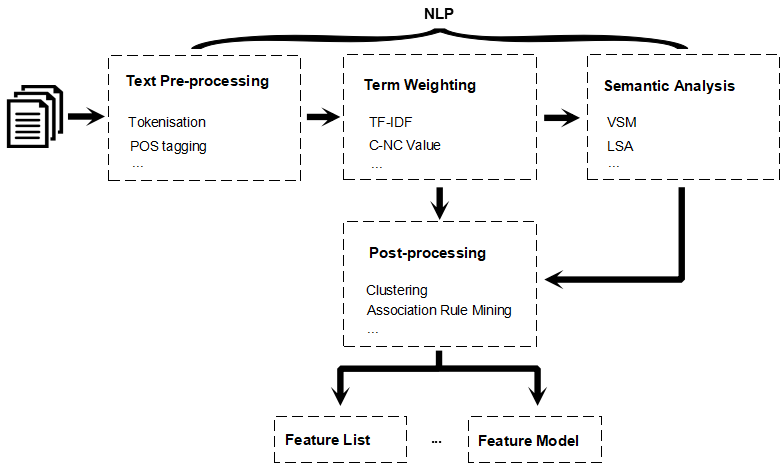
\includegraphics[scale=0.55]{fig_nlp2}
\caption{example graphic, showing a general NLP process for variability extraction}
\label{fig:nlp-general}
\end{figure}

Firstly, NL documents are pre-processed by implementing tokenization, assigning parts of speech to each word, removing stop words and so on, which is named \emph{Text Pre-processing}. Given a character sequence, tokenization is the task of breaking up it into pieces, such as words, symbols and other elements called tokens, which makes it easy for computers to identify and analyze NL documents. Meanwhile, these tokens can be tagged with their type of word (e.g., noun, verb, object, etc.) through using Part-Of-Speech tagging (POS tagging). Lemmatization can be used to transform different forms of a word into the common base form of the word. For example, the semantically related words, "activates", "activated", "activating", with similar meaning are able to be converted into the word "activate". Additionally, stop words which usually refer to the most common words in a vocabulary (e.g., "the", "at", "a") are removed in this phase, as they lack any linguistic information. Certainly, there doesn't exist a single universal list of stop words, which are able to be selected in terms of the specific given purpose. An example for tokenization is as follows:

\definecolor{shadecolor}{rgb}{0.92,0.92,0.92}
\begin{shaded}
\begin{itemize}
    \item [Requirement:] "When the alarm system is activated, this is indicated by the light of the LED."
    \item [Tokenization:] 'When', 'the', 'alarm', 'system', 'is', 'activated', ',', 'this', 'is', 'indicated', 'by', 'the', 'light', 'of', 'the', 'LED', '.'
\end{itemize}
\end{shaded} 

Secondly, some \emph{Term weighting} techniques are typically used to assess the importance of terms in NL documents usually based on the numerical statistics, such as, computing the the frequency of their occurrence in different NL documents. Term Frequency-Inverse Document Frequency (TF-IDF) and C-NC value are two commonly used techniques. 
Generally speaking, TF-IDF relies on the term frequency in a given document and inverse document frequency in a collection as a whole, in which the term is considered significant if it appears frequently in a document, but infrequently in other documents. Meanwhile, C-NC value is a more sophisticated statistical measure which combines linguistic and statistical information. 

Thirdly, \emph{Semantic Analysis} sometimes are applied to achieve the semantic information of the NL documents. Several techniques, such as, Vector Space Model (VSM) and Latent Semantic Analysis (LSA) are widely used to conduct a semantic analysis. Actually, semantic analysis in this context mostly refers to distributional semantics research filed analyzing the semantic similarities between linguistic items in terms of the corresponding word vector similarity, while the vector representation is calculated and modelled by words distributional properties in NL documents. Moreover, the cosine value between the vectors are typically used to measure the similarity called cosine similarity.

Finally, except for the  general NLP process, a \emph{post-processing} step is indispensable to further analyze the processed NL documents with specific focus on identifying features and extracting variation points. Certainly, various techniques regarding information retrieval and machine learning can be used in this step, such as, Clustering Approaches and Association Rule Mining. Cluster approaches are adopted to group similar features with a feature being a cluster of tight-related requirements. Association rule mining is used to discover affinities among features across products, and to augment and enrich the initial product profile. In addition, there are also some rule-based methods in terms of the transformed data by NLP. 

After post-processing, various outputs can be achieved in terms of different given topics, such as, a feature list, some variation points or feature model. The NLP techniques that are able to be applied in this research area are not limited to aforementioned methods. Moreover, advances in NLP, information retrieval, deep learning promote the development of feature and variability extraction from NL documents in SPLs.

\section{Feature Extraction}
\label{sec:feature}
\index{Feature}
% 1. feature
%   similarity-based method 
% 2. feature terms (i.e., feature naming)
% 3. traceability link between different artifacts


Feature is the initial artifact in a feature model. Diverse approaches have been utilized for extracting features from NL documents, while we mainly introduce three kinds of mostly used methods concluded as similarity-based method, graph-based method and feature terms extraction.

\subsection{Similarity-Based Feature Extraction}
% 1. semantic model
% Traditional Distributional Semantic Models
% 2. similarity metric
% 3. clustering

similarity-based feature extraction is the most popular method.
The similarity information among words and sentences is an indispensable property which is able to be analyzed and utilized for feature extraction from NL documents.
In order to achieve the similarity value of each pair of the words, sentences or requirements, various similarity measures are able to be applied, such as, string-based, corpus-based and knowledge-based similarities \cite{WaelA13}. However, the mostly used similarity measures in the context of feature extraction from requirements are \textit{corpus-based} and \textit{knowledge-based} similarities \cite{LiSS17}. The reason is that the similarity value of each pair of the requirements highly depend on the semantic information of the requirements, while string-based similarity measure lack the capability of achieving accurate semantic information.

\begin{figure}
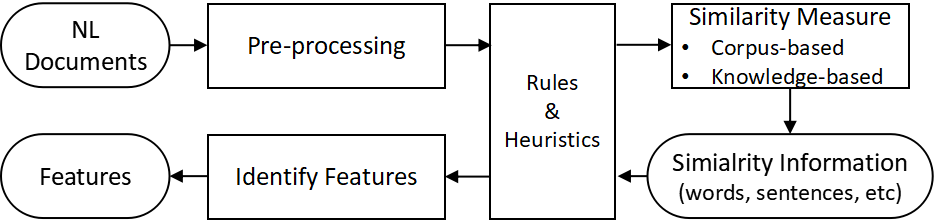
\includegraphics[scale=0.4]{figs/similar_feature.png}
\caption{A general process for similarity-based feature extraction}
\label{fig:similar_feature}
\end{figure}

Fig. \ref{fig:similar_feature} shows the general work flow regarding similarity-based feature extraction. Initially, except for tokenization , lemmatization and removing stop words, a POS filter is common to be used in order to select the most meaningful words, such as nouns, adjectives and verbs. After pre-processing step, different similarity measures can be applied to achieve the similarity information including similarity values and similarity matrix regarding words, sentences, or requirements. Then, the similarity information will be further analyzed by different approaches, such as clustering algorithms or even manual analysis. Certainly, \textit{clustering algorithms} are most popular methods to automate the analysis, where similar information (e.g., words, sentences, requirements) are grouped in terms of the \textit{similarity matrix} of the requirements. Finally, the features can be identified by the clusters (i.e., groups of similar information), taking different rules or heuristics into account.

\subsubsection{Similarity Measure}
\textit{\textbf{Corpus-based similarity.}}
The semantic similarities of words, sentences or texts are obtained in terms of a numeric representation learned from the semantic information of a large text collections, called corpus-based similarity. In our case, the corpora can be any text collections regarding the products or systems in a specific domain, such as SRS. There are two kinds of corpus-based similarity measure regularly used to achieve the similarity: traditional distributional semantic models (DSMs) and neural word embedding.

\textit{Traditional DSMs} can be considered as count models, since they operate on co-occurrence matrices to initialize the vector representations of words, such as counting co-occurrences of words appearing in a specific corpus. VSM and LSA are the common traditional DSMs applied in the research area for feature extraction from requirements \cite{KumakiTWF12,AlvesSBRSRPR08,WestonCR09}.

\textit{Neural word embedding} is a neural-network-based natural language processing architecture which can be seen as predict models, since the vector representations of words or texts can be gained from a pre-trained language model trained on a large text collections. There are also various techniques supporting to achieve accurate neural word embedding models, such as word2vec, Glove and FastText \todo{citations}. \todo{Neural word embedding for feature extraction}

\textit{\textbf{Knowledge-based similarity.}}
The similarities among words depend on the degree of the words' semantic relatedness drawn from semantic networks or knowledge bases, called knowledge-based similarity \todo{citation}\cite{Corpus-based and Knowledge-based Measures of Text Semantic Similarity}. WordNet as a large Knowledge base has been extensively used to achieve the semantic relatedness of words in various research areas. It is a large lexical database of English in which nouns, verbs, adjectives and adverbs are grouped into sets of cognitive synonyms, each expressing a distinct concept \cite{Miller95}. In WoerdNet, synsets denote the sets of cognitive synonyms, interlinked by means of conceptual-semantic and lexical relations. There exist some approaches for feature extraction by using WordNet to identify synonyms and compute the similarity~\cite{ItzikR14,ItzikRBW16,Wang15,Wang16}.

\subsubsection{Rules \& Heuristics}
\todo{rethink this subtitle}
The rule-based methods and heuristics are typically used to analyze and process the requirements in order to extract features, taking the different kinds of similarity information into account.

\textit{\textbf{Semantic roles.}} 
In some research works \todo{citation}\cite{ItzikR14,ReinhartzIW14}, the requirements are further analyzed and processed to extract some predicated semantic roles (e.g., agent, action, Object, ect) from each individual requirement based on Semantic Role Labelling (SRL) technique. The similarity of each pair of the requirements relies on the weighted average similarity of the predicated semantic roles in the requirements.

\textit{\textbf{Clustering algorithms.}}
The widely used methods to analyze the similarity information automatically are clustering algorithms, such as, K-means, hierarchical clustering and DBSCAN. The indispensable assumption is that For example, if we assume that several requirements related to the similar functionality belong to a particular feature, we can observe that a cluster denotes a feature.

\subsection{Graph-Based Feature Extraction}


Graph-based approaches are able to applied for feature extraction. In graph theory, a graph is a network of a set of objects, while some pairs of objects are somehow related with each other. Generally, we use vertices (i.e., points or nodes) to represent the objects and use edges (i.e., lines) to present the correlation of the pairs of vertices. In other words, a graph is a set of vertices connected with edges. In the context of SPLs, a graph G = (V,E) in which vertex V and edge E can be defined as diverse forms. There are different types of graphs, such as undirected graph and directed graph. We briefly introduce an application of undirected graph for feature extraction in terms of research work \cite{ChenZZM05}:

\textit{\textbf{Undirected graph.}} Chen et al. utilized a undirected graph to illustrate some dedicated relationships between individual requirements. In this graph, vertices denotes individual requirements, while edges represent the dedicated relationships between pairs of requirements. Meanwhile, the weight of each edge is used to measure the the strength of the relationships between requirements. After the graph construction, features are clustered by the size of weight values.

Moreover, the graph-based method is not only able to identify features, but also capable of extracting variability information (cf. Section \ref{sec:variability}), especially for the application of \textit{directed graph}.

% 1. features are clustered by the weights between two requirements in an undirected graph. \cite{ChenZZM05}

% \textit{\textbf{Directed graph.}}
% 2. Association rule mining. \cite{DavrilDHACH13}

% 3. \cite{AcherCPHVCL12}

\subsection{Feature Term Extraction}
In NL documents, there have already existed some domain specific terms representing the concrete functionality in a system. Hence, it's possible to use the specific term to denote a feature, called \textit{feature term}.
For example, in the requirement below:
\definecolor{shadecolor}{rgb}{0.92,0.92,0.92}
\begin{shaded}
"The \underline{interior monitoring} is deactivated as soon as the \underline{alarm system} is deactivated."
\end{shaded}
Since the terms, "interior monitoring" and "alarm system", denote the specific functionality in current system, "interior monitoring" and "alarm system" can be regarded as feature terms. These feature terms not only can represent the feature names, but also can be used to detect the variability information, taking the syntax of the requirements into consideration. 

There are different NLP techniques capable of extracting feature terms, such as keyword extraction, Named Entity Recognition (NER). In the SPLs context, \textit{POS pattern} is common keyword extraction method to identify the meaningful terms, for example, "alarm system" can be identified by a \textit{<noun, noun>} pattern, "interior monitoring" is able to be extracted by a \textit{<adj, noun>} pattern. NER technique is utilized for identifying the named entities of things in the NL documents, such as people and organization names, or gene and protein names. In the SPLs context, feature term is regarded as a named entity. Since we lack open source pre-trained NER models for feature term extraction, we must firstly train a NER model by using a labelled dataset. 




\section{Variability Extraction}
\label{sec:variability}
\index{Variability}
\todo{}
\subsection{Optionality}
Diverse approaches are utilized to detect the optionality (i.e., mandatory and optional).

\textit{\textbf{Occurrence.}} \todo{rethink the subtitle}The most popular method is to apply heuristics or pre-defined rules to detect the optionality based on the occurrence of requirements or domain-specific terms in different variants. 
For example, we can simply define a rule that if a feature extracted from some requirements and these requirements come from all the variants, the feature is mandatory; otherwise, the feature is optional. Although the rules vary with different research topics, the foundation of the rules is the distribution of features in different variants which can be named the traceability link between features and variants.

The general process is that: a) if the dataset of requirements contains the corresponding variants information, we can directly obtain a mapping between requirements and variants; b) after feature extraction, the approach we used is capable of achieve a mapping between features and requirements; c) based on the aforementioned two mappings, we can achieve a traceability link between feature and variants; d) in terms of the distribution of features in different variants, which means we know whether a variant includes a certain feature or not, different methods such as heuristics can be applied to extract the optionality. What should be highlighted here is that: the two-mapping is a bridge used to connect the features and variants and the bridge is possible to be constructed by other mappings, such as the mapping between domain-specific terms and variants \cite{FerrariSD13}. 
The underlying idea is that the distribution of different features in different variants can be regarded as a kind of domain knowledge, while we use statistics to quantify this kind of domain knowledge in order to further detect the optionality.

% 1. Occurrence in variants. mandatory and optional is extracted by calculating the occurrence of dedicated attribute \cite{ChenZZM05} or artifacts (requirements \cite{SPLC paper} \cite{WestonCR09} \cite{ItzikR14} , domain-specific terms \cite{FerrariSD13}).  

\textit{\textbf{Lexical analysis.}} Another regularly applied method is to analyze some specific words appearing in the requirements, such as adjectives (e.g., "possible"), model verbs (e.g., "must"), adverbs (e.g., "optionally") and etc.. 
For example, in the requirement below \cite{Sree-KumarPC18}:
\definecolor{shadecolor}{rgb}{0.92,0.92,0.92}
\begin{shaded}
"The \underline{publishing module} \textit{\textbf{can}} be configured using a \underline{custom reports module}." 
\end{shaded}

The model verb "can" represent a possibility, from which the relationship between the two feature terms, "publishing module" and "custom reports module", are able to be deduced as optional.


% 2. Lexical analysis. The determination of whether a feature is optional, alternative, or or-feature is performed by analyzing the context of its requirements by searching for words denoting these concepts (e.g., "optionally", "alternatively", "at least one of"). \cite{AlvesSBRSRPR08} \cite{Laura's VaMos paper} \cite{AcherCPHVCL12} 
%  \cite{P2 see excel sheet} defined some rules in terms of the occurrence and position of some special words

\textit{\textbf{Association rule mining.}} The optionality can also be detected by the associations between features based on association rule mining, one of the data mining techniques. For example, Davril et al. proposed to use an implication graph, a directed graph, where vertex denotes a feature and edge denotes the confidence between the two connected features to determine whether a feature is mondatory or not \cite{DavrilDHACH13}.

% 3. Association rule mining. \cite{DavrilDHACH13}


% 4. \cite{HamzaW15} mandatory and optional features are identified by heuristics (actor, action, and object)

\subsection{Group Constraints}
The methods for group constraints (e.g., Or-Group and XOR-Group) extraction are predominantly related to the techniques used for optionality extraction.

\textit{\textbf{Occurrence.}} For the example, in the research work of Itzik et al. \cite{ItzikR14}, feature model are generated by grouping similar requirements based on hierarchical clustering algorithm, including some abstract and concrete features. Meanwhile, in their model, each concrete feature denotes an individual functional requirement. Moreover, two rule are pre-defined for group constraints extraction:

\definecolor{shadecolor}{rgb}{0.92,0.92,0.92}
\begin{shaded}
\begin{itemize}
    \item [1.] If at least two requirements that are grouped under the same parent node appear in the same input document, then the corresponding requirements are \textit{OR-grouped}.
    \item [2.] If requirements originating from different input files are grouped under the same parent node, we consider the corresponding requirements as \textit{XOR-grouped}.
\end{itemize} 
\end{shaded}
In the aboved two rules, the input documents/files can be regarded as variants. The parent node represents an abstract feature, while each requirement represents a concrete feature. Hence, we can observe that the distribution of features in variants is also capable of being applied to extract the group constraints. Moreover, other different rules are defined in paper \cite{LiSS18}.


% 1. Occurrence in variants. \cite{ItzikR14} \cite{SPLC aper}

\textit{\textbf{Lexical analysis.}} For extracting group constraints based on lexical analysis, we also illustrate an example from Sree-Kumar et al. research work \cite{Sree-KumarPC18}:
\definecolor{shadecolor}{rgb}{0.92,0.92,0.92}
\begin{shaded}
"We believe that \underline{proof of individuality (POI)} \textit{\textbf{can}} be better solved with \underline{biometrics} than what is currently being proposed in the Ethereum community - \underline{a series of video calls}."
\end{shaded}
We can deduce that there two potential sub-features, "biometrics" and "a series of video calls", belonging to "proof of individuality". In terms of specific model verb "can", we observe that the two sub-features may or may not coexist when the parent feature is configured. Hence, the two sub-features are possibly or-grouped.

% 2. Lexical analysis. The determination of whether a feature is optional, alternative, or or-feature is performed by analyzing the context of its requirements by searching for words denoting these concepts (e.g., "optionally", "alternatively", "at least one of"). \cite{AlvesSBRSRPR08}

\textit{\textbf{Association rule mining.}} As the aforementioned optionality extraction based on implication graph drawn by association rule mining \cite{DavrilDHACH13}, the or-group relation is also detected by the vertex (i.e., concrete feature) of implication graph. If an abstract feature can be comprised of concrete features from the vertices in the implication graph, these concrete features are regarded as or-grouped features.

% 3. Association rule mining. \cite{DavrilDHACH13}
% 4. \cite{AcherCPHVCL12}

\subsection{Cross-Tree Constriants}

\textit{\textbf{NER.}} We have known that NER can be used to extract features, while it's certainly possible to applied NER technique to detect cross-tree constraints. Firstly, if there is no pre-trained NER model, we need to train a NER model by a labelled dataset. In this labelled dataset, the requirements containing specific cross-tree constraints are assigned a dedicated label. An example of labelled requirements \cite{BagheriEG12} is shown below:

\definecolor{shadecolor}{rgb}{0.92,0.92,0.92}
\begin{shaded}
"A graph cannot be both directed and undirected" and "A graph can either be weighted or unweighted" are labelled as \textit{\textbf{ic}}.
\end{shaded}
The label \textit{ic} denotes integrity constraints (i.e., cross-tree constraints). The label is just symbol used to present that there are potential cross-tree constraints in the requirements.

% 1. NER \cite{BagheriEG12}

% 2. Association rule mining. \cite{DavrilDHACH13}

\section{Challenges and Risks}
\label{sec:challenge}
\index{Challenge}
% Always give a unique label
% and use \ref{<label>} for cross-references
% and \cite{<label>} for bibliographic references
% use \sectionmark{}
% to alter or adjust the section heading in the running head



\bibliographystyle{spmpsci}
\bibliography{Requirements-Schulze} 
\end{document}
